\documentclass[10pt,a4paper]{article}
\usepackage[utf8]{inputenc}
\usepackage[german]{babel}
\usepackage{mathrsfs}
\usepackage{amsmath}
\usepackage{amsfonts}
\usepackage{amssymb}
\usepackage{amsthm}
\usepackage{graphicx}
\usepackage{float}
\usepackage[left=2cm,right=2cm,top=2cm,bottom=2cm]{geometry}

\begin{document}

\section{Aufgabe 1}
\begin{proof}
  Sei $k$ der gesuchte Schlüssel und $a$ ein Array der Länge $n$.
  Ich zeige per Induktion über $n$, dass die binäre Suche den Index des Elements mit dem Schlüssel $k$ zurückgibt, wenn es enthalten ist, und sonst $-1$ als Fehlerwert.
  Dabei werde ich $k$ synonym für den Schlüssel und das Element mit diesem Schlüssel verwenden.
  Außerdem bezeichne ich mit links ``in Richtung der kleineren Indizes'' und mit rechts ``in Richtung der größeren Indizes''.

  Sei $n = 0$.
  Das Array ist leer, sodass $k$ offensichtlich nicht enthalten sein kann und $-1$ zurückgegeben wird.

  Sei $n = 1$.
  Das Array enthält genau 1 Element.
  Wenn dieses $k$ ist, gibt die Suche $0$ zurück, sonst $-1$.

  Sei $n > 1$ und die Behauptung für alle $m < n$ bereits gezeigt.
  Dann wählt der Algorithmus das Element $m = a[\lceil \frac{N - 1}{2} \rceil]$ aus.
  Ist $m.k = k$, so wird $\lceil \frac{N - 1}{2} \rceil$ zurückgegeben und $a[\lceil \frac{N - 1}{2} \rceil] = m = k$.
  Ist $m.k > k$, so kann es sich nur im linken Teil $a[0 .. \lceil \frac{N - 1}{2} \rceil - 1]$ des Arrays befinden.
  Da dieser Teil $m$ nicht enthält, ist er kürzer als das Originalarray, sodass die Binärsuche darauf angewendet werden kann und den Wert $i$ zurückgibt.
  Wenn $i = -1$, ist $k$ nicht im linken Teil und somit auch nicht in $a$ und die Suche gibt $-1$ zurück.
  Sonst wurde $k$ gefunden und befindet sich an Position $i$, was dann auch der Rückgabewert ist, weil $a[i] = k$.
  Ist $m.k < k$, so kann sich $k$ nur im rechten Teil $a[\lceil \frac{N - 1}{2} \rceil + 1 .. N - 1]$ befinden.
  Aus dem selben Grund wie im anderen Fall, kann man auch hier die Suche anwenden und erhält den Rückgabewert $i$.
  Ist $i = -1$, so ist $k$ nicht im rechten Teil und somit auch nicht in $a$.
  Also wird $-1$ zurückgegeben.
  Ansonsten ist $k$ an Position $i$ in der rechten Hälfte.
  Damit befindet sich $k$ an der Position $\lceil \frac{N - 1}{2} \rceil + 1 + i$ in $a$, sodass diese zurückgegeben wird.
\end{proof}

\section{Aufgabe 2}
Zuerst wird mit $10$ verglichen und danach schon mit $18$, was die Suche beendet und $6$ zurückgibt.

\section{Aufgabe 3}

\subsection{Sequentiell und Binär}
\begin{equation}
  k = 1
\end{equation}
\begin{equation}
  A_{1} = 1\ 2\ 3
\end{equation}
\begin{equation}
  A_{2} = 0\ 1\ 2
\end{equation}

\subsection{Sequentiell und Fibonacci}
\begin{equation}
  k = 1
\end{equation}
\begin{equation}
  A_{1} = 1\ 2\ 3\ 4
\end{equation}
\begin{equation}
  A_{2} = 0\ 1\ 2\ 3
\end{equation}

\subsection{Sequentiell und Interpolation}
\begin{equation}
  k = 100
\end{equation}
\begin{equation}
  A_{1} = 0\ 100\ 102\ 103\ 104\ 105\ 106\ 107
\end{equation}
\begin{equation}
  A_{2} = 99\ 100\ 101
\end{equation}

\subsection{Binär und Fibonacci}
\begin{equation}
  k = 4
\end{equation}
\begin{equation}
  A_{1} = 1\ 2\ 3\ 4\ 5\ 6\ 7
\end{equation}
\begin{equation}
  A_{2} = 2\ 3\ 4\ 5\ 6\ 7\ 8
\end{equation}

\subsection{Binär und Interpolation}
\begin{equation}
  k = 10
\end{equation}
\begin{equation}
  A_{1} = 0\ 5\ 10\ 50\ 100
\end{equation}
\begin{equation}
  A_{2} = 0\ 10\ 20\ 30\ 50
\end{equation}

\subsection{Fibonacci und Interpolation}
\begin{equation}
  k = 10
\end{equation}
\begin{equation}
  A_{1} = 0\ 1\ 10\ 11\ 12\ 13\ 70
\end{equation}
\begin{equation}
  A_{2} = 7\ 8\ 9\ 10\ 11\ 12\ 13
\end{equation}

\section{Aufgabe 4}
Die Schlüssel beginnen bei 1 und die X-Blätter habe ich eingefügt, um explizit anzuzeigen, dass die Suche auf der linken Seite erfolglos beendet wird.
\begin{figure}[H]
  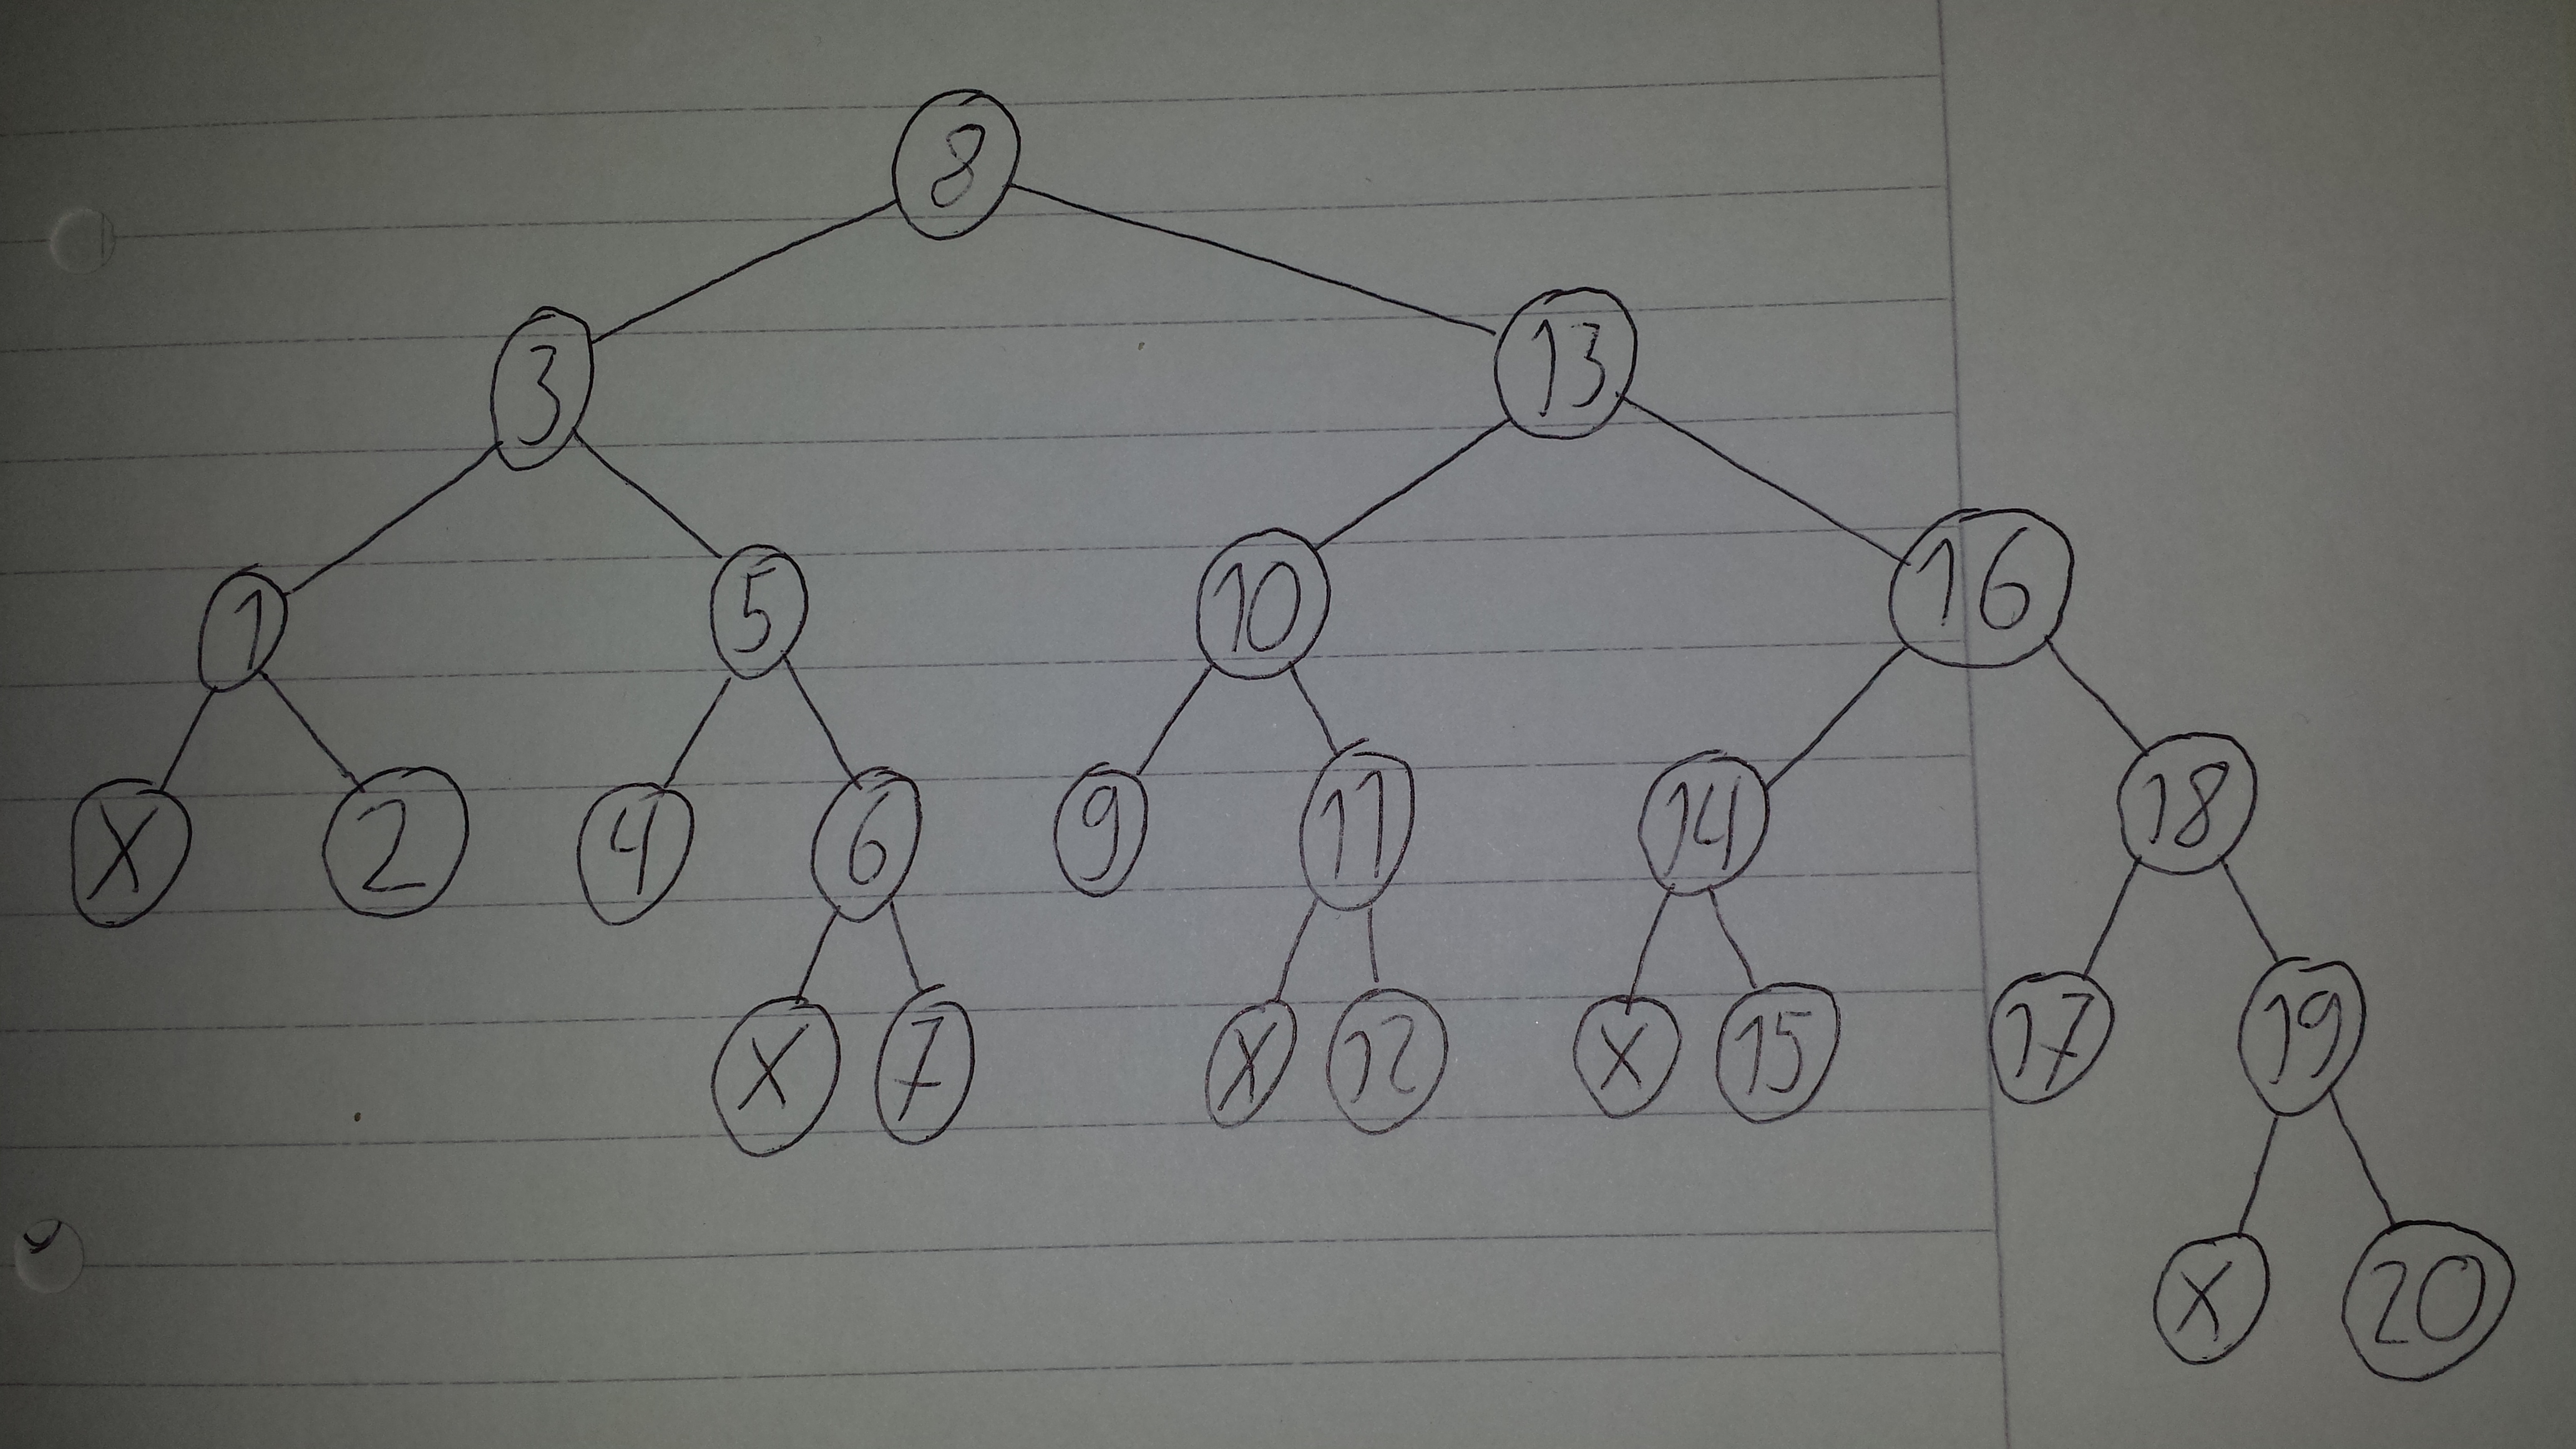
\includegraphics[width=400pt]{6_4}
\end{figure}

\end{document}